% Project report: P27 Self-Supervised Contrastive Pretraining when Labels are Scarce
% Build: tectonic main.tex   (or: pdflatex main.tex, run twice)
\documentclass[11pt,a4paper]{article}
\usepackage[margin=2.5cm]{geometry}
\usepackage[T1]{fontenc}
\usepackage{lmodern}
\usepackage{microtype}
\usepackage{amsmath,amssymb}
\usepackage{graphicx}
\usepackage{booktabs}
\usepackage{float}
\usepackage[round]{natbib}
\usepackage[hidelinks]{hyperref}
\graphicspath{{../results/}}
\setlength{\parskip}{4pt}

\title{Self-Supervised Contrastive Pretraining when Labels are Scarce:\\SimCLR on STL-10}
\author{Shubham Kang \quad Sandhya Parmar \quad Nidhi\\[4pt]
\small Code: \url{https://github.com/ShubhamKang/SimCLR-Deep-Learning}}
\date{November 2026}

\begin{document}
\maketitle

% ---------------------------------------------------------------- Abstract (Shubham)
\begin{abstract}
Labelled data is expensive, while unlabelled images are easy to collect. We study whether self-supervised
contrastive pretraining with SimCLR lets a classifier reach good accuracy with far fewer labels, and which
data augmentations matter most when compute is limited. Using STL-10, we pretrain a ResNet-18 encoder on
100,000 unlabelled images for 50 epochs on a single GPU, then train classifiers on 100\%, 20\%, 10\% and 1\%
of the 5,000 labelled training images. With 10\% of the labels, a supervised ResNet-18 trained from scratch
reaches 44.3\% test accuracy, while a linear probe on the SimCLR encoder reaches 65.2\% and fine-tuning
reaches 65.5\%. With only 1\% of the labels (50 images), the linear probe reaches 53.1\%, double the
baseline's 26.8\%. An ablation over five augmentations on a short 20-epoch schedule shows that random resized
crop matters most: removing it lowers linear-probe accuracy from 57.0\% to 38.2\%, close to using no
augmentation at all (36.9\%). Colour jitter ($-7.0$ points) and grayscale ($-5.8$) come next, while flip and
blur give no measurable benefit on this budget. Smaller batches did better at a fixed number of epochs:
59.3\% at batch size 64 versus 53.2\% at 512.
\end{abstract}

% ---------------------------------------------------------------- 1. Introduction (Nidhi)
\section{Introduction}
Deep learning models for image classification have achieved strong results, but their success has
historically depended on large amounts of labelled data. Collecting and annotating labels at scale is
expensive and time-consuming, which makes this dependence a practical barrier in many real-world settings.
Medical imaging, satellite analysis and rare-event detection all face situations where unlabelled images are
plentiful but labelled examples number in the tens or hundreds.

This project examines one concrete instance of that problem: how accurately can a classifier be trained on
STL-10 when only a small fraction of the available labels is used, and can self-supervised pretraining on the
unlabelled images close the gap?

The STL-10 dataset \citep{coates2011} is designed for this setting. It provides 100,000 unlabelled images
alongside a small labelled training set of 5,000 images (500 per class across 10 categories), and a test set
of 8,000 images. We study label fractions of 100\%, 20\%, 10\% and 1\%, corresponding to 5,000 down to just 50
labelled training images, a regime where supervised training from scratch degrades sharply.

Our approach is SimCLR (Simple Framework for Contrastive Learning of Visual Representations)
\citep{chen2020}, which learns visual features from unlabelled images by training a network to produce similar
representations for two augmented views of the same image and dissimilar representations for views of
different images. The learned encoder is then transferred to the classification task with a small labelled set.

We investigate two aspects of SimCLR that are practically important on a limited compute budget:
\begin{enumerate}
  \item \textbf{Which augmentations matter most?} SimCLR relies heavily on the composition of image
  augmentations to define the self-supervised task. We run a leave-one-out and single-augmentation ablation
  across five augmentations (random crop, horizontal flip, colour jitter, grayscale and Gaussian blur) to
  measure the contribution of each.
  \item \textbf{How does batch size affect the learned representations?} The contrastive loss treats every
  other image in the same batch as a negative example, so larger batches provide more negatives and
  potentially a stronger learning signal. We train with batch sizes of 64, 128, 256 and 512 on a fixed short
  schedule to isolate the effect of batch size under a constant compute budget.
\end{enumerate}

Section~\ref{sec:related} reviews related work. Section~\ref{sec:method} describes SimCLR and our training
procedure, and Section~\ref{sec:setup} the experimental setup. Section~\ref{sec:results} compares the
supervised baseline with SimCLR. Sections~\ref{sec:aug} and~\ref{sec:bs} present the augmentation and
batch-size ablations, Section~\ref{sec:discussion} discusses limitations, and Section~\ref{sec:conclusion}
concludes.

% ---------------------------------------------------------------- 2. Related work (Nidhi)
\section{Related work}\label{sec:related}

\subsection{Supervised baselines for image classification}
Convolutional neural networks trained end to end with cross-entropy loss on labelled data have been the
standard approach to image classification since AlexNet \citep{krizhevsky2012}. ResNet architectures
\citep{he2016} introduced residual connections that allow very deep networks to be trained reliably, and
ResNet-18 remains a common choice for small and medium datasets. The core limitation of fully supervised
training is its need for data: accuracy falls quickly when fewer labels are available, particularly below
10\% of the training set, because the network overfits the small labelled set instead of learning features
that generalise.

\subsection{Self-supervised and contrastive learning}
Self-supervised learning avoids the label bottleneck by constructing a pretext task directly from unlabelled
data. Early pretext tasks included predicting image rotations \citep{gidaris2018}, solving jigsaw puzzles
\citep{noroozi2016} and colourisation \citep{zhang2016}. These tasks produced transferable features but were
often brittle and task-specific.

Contrastive learning unified these ideas under one objective: pull together representations of related pairs
and push apart unrelated ones. Instance discrimination \citep{wu2018} treated each image as its own class and
used a memory bank of negatives. Momentum Contrast (MoCo) \citep{he2020} replaced the memory bank with a
momentum encoder and a queue, decoupling batch size from the number of negatives. Contrastive Predictive
Coding (CPC) \citep{oord2018} learned representations by predicting future parts of a sequence in a learned
latent space with a similar contrastive objective.

\subsection{SimCLR}
SimCLR \citep{chen2020} simplified the contrastive learning pipeline while achieving state-of-the-art results
at the time of publication. Its key elements are:
\begin{itemize}
  \item \textbf{Two-view augmentation.} Each training image is augmented twice with a stochastic pipeline
  (crop, flip, colour jitter, grayscale, blur) to form a positive pair. All other images in the same batch
  form negative pairs.
  \item \textbf{Projection head.} A two-layer MLP is placed on top of the encoder during pretraining. Computing
  the contrastive loss on the head's output, and discarding the head afterwards, improves the encoder's
  representations for downstream tasks.
  \item \textbf{NT-Xent loss.} The normalised temperature-scaled cross-entropy loss treats the task as a
  classification problem: for each of the $2N$ views in a batch, the network must identify its one positive
  partner among the $2N-1$ other views.
  \item \textbf{Large batch size.} The original ImageNet results used batch sizes of 4,096 or 8,192 with the
  LARS optimiser \citep{you2017}, exploiting the fact that more negatives per image strengthen the contrastive
  signal. This motivates our batch-size ablation.
\end{itemize}
The SimCLR paper found that the composition of augmentations is one of the most important design choices,
and that random cropping combined with colour distortion is the key pair for ImageNet linear evaluation. We
test this finding on STL-10 under a small compute budget.

\subsection{Linear evaluation and fine-tuning}
A standard way to measure the quality of self-supervised representations is linear evaluation: freeze the
pretrained encoder and train only a linear classifier on top of it. A good encoder produces linearly separable
features without task-specific training. Fine-tuning, which starts from the pretrained encoder and updates all
weights, usually gives higher accuracy but needs more labelled data to avoid overfitting. Comparing the two
shows how much of the gain comes from adapting the encoder and how much from the fixed features.

\subsection{STL-10 benchmark}
STL-10 \citep{coates2011} was designed as a benchmark for self-supervised and semi-supervised methods. Its
$96\times96$ colour images are larger than those of CIFAR-10, and the 100,000 unlabelled images come from a
broader distribution than the 10 labelled classes, which makes pretraining harder and more realistic. As a
reference point, a public PyTorch SimCLR implementation reports 74.45\% linear-probe accuracy on STL-10 with a
ResNet-18 pretrained for 100 epochs \citep{silva2020}. Our experiments use shorter schedules suited to a
student compute budget and focus on relative comparisons, not state-of-the-art numbers.

% ---------------------------------------------------------------- 3. Method (Shubham)
\section{Method}\label{sec:method}

\subsection{Contrastive pretraining}
We follow SimCLR \citep{chen2020}. For each unlabelled image we draw two random augmentations, giving two views
$x_i$ and $x_j$. A ResNet-18 encoder $f$ maps each view to a 512-dimensional feature vector $h$, and a two-layer
MLP projection head $g$ (512--512--128 with a ReLU) maps $h$ to $z$. In a batch of $N$ images, the two views of
the same image form a positive pair and the other $2(N-1)$ views are negatives. The NT-Xent loss for a positive
pair $(i,j)$ is
\begin{equation}
  \ell_{i,j} = -\log \frac{\exp(\mathrm{sim}(z_i, z_j)/\tau)}{\sum_{k=1}^{2N} \mathbb{1}_{[k \neq i]}\exp(\mathrm{sim}(z_i, z_k)/\tau)},
\end{equation}
where $\mathrm{sim}$ is cosine similarity and $\tau = 0.5$ is the temperature. The loss is averaged over all
$2N$ views. After pretraining the projection head is discarded and only the encoder $f$ is kept.

\subsection{Augmentations}
The five augmentations are random resized crop (scale 0.2 to 1.0), horizontal flip ($p=0.5$), colour jitter
(brightness, contrast and saturation 0.4, hue 0.1, applied with $p=0.8$), random grayscale ($p=0.2$) and
Gaussian blur (kernel size 9, $\sigma \in [0.1, 2.0]$, $p=0.5$). Each one can be switched on or off
independently, which is what the ablation uses. When crop is off, images are only resized.

\subsection{Training details}
The encoder is a ResNet-18 with random initialisation and $96\times96$ inputs. We use AdamW
\citep{loshchilov2019} with learning rate $3\times10^{-4}$ and weight decay $10^{-6}$, cosine learning-rate
decay and mixed precision. The main model is trained on all 100,000 unlabelled images with batch size 256 for
50 epochs, which took 3.1 hours on one Kaggle Tesla T4 GPU. Figure~\ref{fig:loss} shows the loss, which fell
from 5.12 to 4.58 and changed by less than 0.01 over the last ten epochs. The ablations use a shorter, identical
schedule: 20 epochs on a fixed 20,000-image subset, so that each run takes 4 to 16 minutes.

\begin{figure}[H]
  \centering
  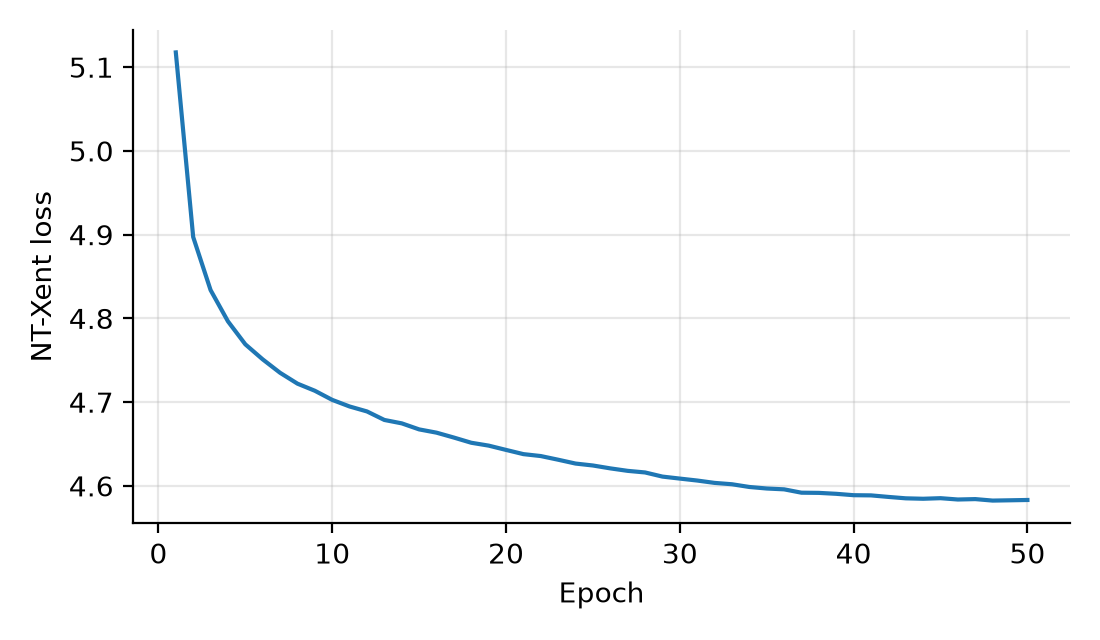
\includegraphics[width=0.6\linewidth]{pretrain_loss.png}
  \caption{NT-Xent loss during the 50-epoch SimCLR pretraining on 100,000 unlabelled images.}
  \label{fig:loss}
\end{figure}

% ---------------------------------------------------------------- 4. Experimental setup (Sandhya)
\section{Experimental setup}\label{sec:setup}

\subsection{Dataset}
We use STL-10 \citep{coates2011}, which has $96\times96$ colour images in 10 classes (airplane, bird, car,
cat, deer, dog, horse, monkey, ship, truck). It has three parts:
\begin{itemize}
  \item \textbf{Unlabelled split:} 100,000 images, used only for SimCLR pretraining. No labels are used at
  this stage.
  \item \textbf{Train split:} 5,000 labelled images (500 per class), used to train the classifiers.
  \item \textbf{Test split:} 8,000 labelled images (800 per class). Every accuracy in this report is measured
  on the full test set.
\end{itemize}

\subsection{Simulating label scarcity}
We train classifiers on 100\%, 20\%, 10\% and 1\% of the training labels, which is 500, 100, 50 and 5 images
per class (5,000, 1,000, 500 and 50 images in total). Each subset is class-balanced, so a small fraction cannot
miss a class. It is drawn with a fixed random seed (seed 0), so the supervised baseline, the linear probe and
fine-tuning all see exactly the same labelled images at a given fraction.

\subsection{Model}
All methods use the same ResNet-18 encoder with random initialisation (no ImageNet weights). The final
classification layer is removed, so the encoder outputs a 512-dimensional feature vector. A linear layer
(512 to 10) on top of the encoder produces the class scores.

\subsection{Methods compared}
\begin{enumerate}
  \item \textbf{Supervised baseline (no pretraining).} The whole network is trained from random weights on the
  labelled subset only, with AdamW (learning rate $10^{-3}$, weight decay $10^{-4}$), 100 epochs, cosine
  learning-rate decay, batch size 128 (capped at the subset size, see Section~\ref{sec:droplast}) and light
  augmentation (random crop after 8-pixel padding, and horizontal flip).
  \item \textbf{SimCLR linear probe.} The pretrained encoder is frozen. Features are extracted once without
  augmentation and standardised using training-set statistics only. A single linear layer is trained with
  full-batch Adam (learning rate $10^{-3}$, weight decay $10^{-4}$) for 300 steps. This measures how linearly
  separable the learned features are.
  \item \textbf{SimCLR fine-tuning.} The pretrained encoder and a new linear layer are trained end to end with
  the same settings as the baseline, except for a smaller learning rate of $3\times10^{-4}$, so that the
  pretrained features are adjusted gently instead of overwritten. Using the same recipe as the baseline makes
  the comparison fair: the only difference is the starting weights.
\end{enumerate}
The ablations in Sections~\ref{sec:aug} and~\ref{sec:bs} are evaluated with the linear probe on 100\% of the
labels.

\subsection{Implementation note: batch size at 1\% labels}\label{sec:droplast}
At 1\% labels the training subset has only 50 images, fewer than the batch size of 128. The original data
loader discarded the last incomplete batch (\texttt{drop\_last=True}). Here that was the only batch, so the
model received no gradient updates and stayed at chance level (about 10\%). We cap the batch size at the size
of the training subset, so every fraction trains for the full 100 epochs.

\subsection{Metric and compute}
The metric is top-1 accuracy on the 8,000 test images. The supervised baseline was trained on a Google Colab
T4 GPU, and SimCLR pretraining, evaluation and ablations on Kaggle T4 GPUs. All results use one seed (seed 0).

% ---------------------------------------------------------------- 5. Results (Sandhya)
\section{Results: supervised baseline vs SimCLR}\label{sec:results}

\begin{table}[H]
  \centering
  \caption{Test accuracy (\%) on STL-10 with different amounts of labelled training data. Best result in each
  row in bold.}
  \label{tab:main}
  \begin{tabular}{lccc}
    \toprule
    Labels used (per class) & Supervised (scratch) & SimCLR linear & SimCLR fine-tune \\
    \midrule
    100\% (500) & 75.5 & 72.6 & \textbf{81.3} \\
    20\% (100)  & 53.4 & 68.6 & \textbf{71.2} \\
    10\% (50)   & 44.3 & 65.2 & \textbf{65.5} \\
    1\% (5)     & 26.8 & \textbf{53.1} & 43.6 \\
    \bottomrule
  \end{tabular}
\end{table}

\begin{table}[H]
  \centering
  \caption{Improvement over the supervised baseline (percentage points).}
  \label{tab:gain}
  \begin{tabular}{lcc}
    \toprule
    Labels used & Linear probe & Fine-tune \\
    \midrule
    100\% & $-2.9$ & $+5.8$ \\
    20\%  & $+15.1$ & $+17.8$ \\
    10\%  & $+20.9$ & $+21.2$ \\
    1\%   & $+26.2$ & $+16.8$ \\
    \bottomrule
  \end{tabular}
\end{table}

\begin{figure}[H]
  \centering
  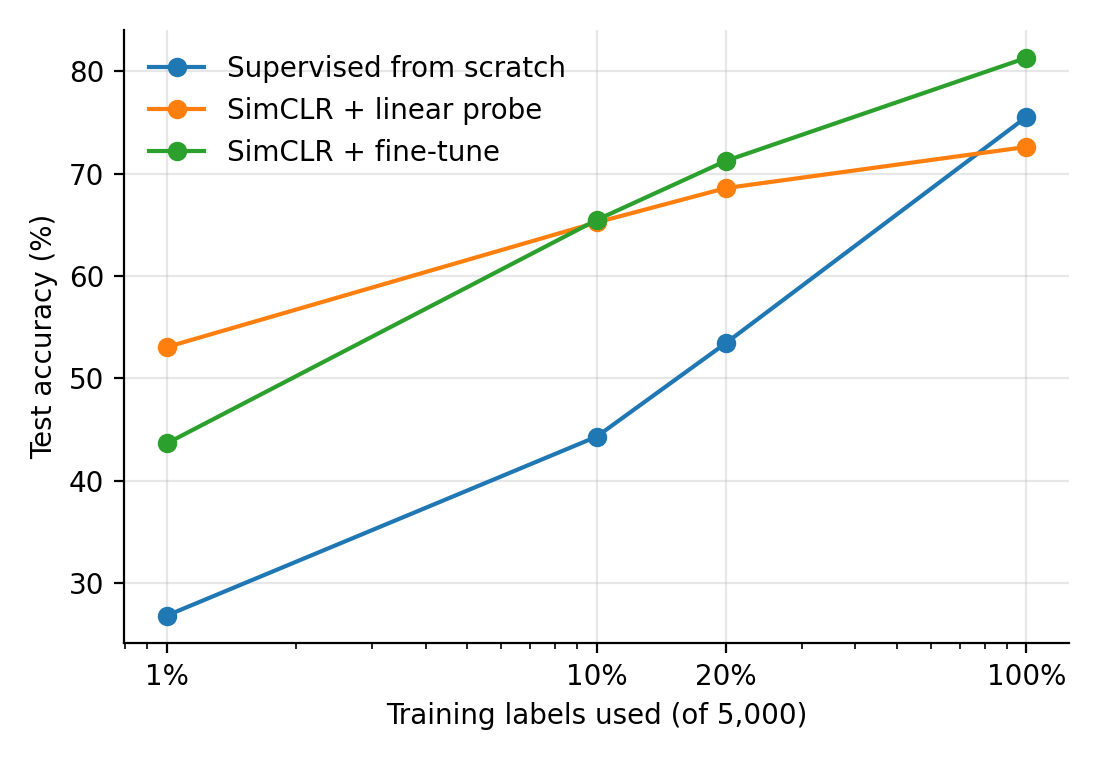
\includegraphics[width=0.65\linewidth]{labels_vs_acc.png}
  \caption{Test accuracy against the fraction of training labels used (log scale).}
  \label{fig:labels}
\end{figure}

\paragraph{Pretraining helps most when labels are scarce.} The supervised baseline loses almost two thirds of
its accuracy as labels go from 100\% to 1\% (75.5\% to 26.8\%). SimCLR is much more robust: the best SimCLR
model drops only from 81.3\% to 53.1\%. The gain over the baseline grows as labels become scarcer, from $+5.8$
points with all labels to $+21.2$ points at 10\% and $+26.2$ points at 1\% (Tables~\ref{tab:main}
and~\ref{tab:gain}, Figure~\ref{fig:labels}).

\paragraph{Label efficiency.} A linear probe trained on just 5 images per class (1\%, 53.1\%) matches the
supervised model trained on 100 images per class (20\%, 53.4\%), about 20 times fewer labels for the same
accuracy. Fine-tuning with 20\% of the labels (71.2\%) comes within 4.3 points of the supervised model trained
on all 5,000 labels (75.5\%).

\paragraph{Linear probe vs fine-tuning.} With 10\% or more labels, fine-tuning is best. Updating the whole
encoder lets it adapt to the classification task, and with all labels it beats the supervised baseline by 5.8
points. At 1\% the order reverses: the linear probe (53.1\%) beats fine-tuning (43.6\%) by 9.4 points. With
only 50 images, training all 11 million parameters for 100 epochs overfits and damages the pretrained
features, while a single linear layer on frozen features cannot overfit as badly. When labels are extremely
scarce, freezing the encoder is the safer choice.

\paragraph{Frozen features with all labels.} With 100\% of the labels the linear probe (72.6\%) is 2.9 points
below the supervised baseline. Frozen features from a 50-epoch pretraining run are not as task-specific as a
network trained end to end on 5,000 labels. The original SimCLR paper pretrains for hundreds of epochs with
much larger batches, and longer pretraining would likely close this gap. Fine-tuning removes the gap entirely.

\paragraph{Caveats.} Each number comes from a single run (seed 0), so differences of about 1 point, such as
linear probe vs fine-tune at 10\% (65.2\% vs 65.5\%), should not be over-interpreted. The trends, however, are
large and consistent across label fractions.

% ---------------------------------------------------------------- 6. Augmentation ablation (Shubham)
\section{Augmentation ablation}\label{sec:aug}
Every run uses the same schedule: 20 epochs of SimCLR pretraining on the same 20,000 unlabelled images
(seed 0), batch size 256, then a linear probe on all 5,000 labels. Table~\ref{tab:aug} and
Figure~\ref{fig:aug} show the results.

\begin{table}[H]
  \centering
  \caption{Augmentation ablation. Linear-probe test accuracy (\%) after 20 epochs of pretraining on 20,000
  images.}
  \label{tab:aug}
  \begin{tabular}{llcc}
    \toprule
    Setting & Augmentations on & Accuracy & Change vs full \\
    \midrule
    full       & crop, flip, colour, gray, blur & 57.0 & -- \\
    no\_crop   & flip, colour, gray, blur & 38.2 & $-18.8$ \\
    no\_color  & crop, flip, gray, blur & 50.0 & $-7.0$ \\
    no\_gray   & crop, flip, colour, blur & 51.2 & $-5.8$ \\
    no\_flip   & crop, colour, gray, blur & 56.9 & $-0.1$ \\
    no\_blur   & crop, flip, colour, gray & 58.6 & $+1.6$ \\
    \midrule
    crop\_color & crop, colour & 53.0 & $-4.0$ \\
    only\_crop  & crop & 45.1 & $-11.9$ \\
    only\_color & colour & 42.7 & $-14.3$ \\
    none        & none & 36.9 & $-20.1$ \\
    \bottomrule
  \end{tabular}
\end{table}

\begin{figure}[H]
  \centering
  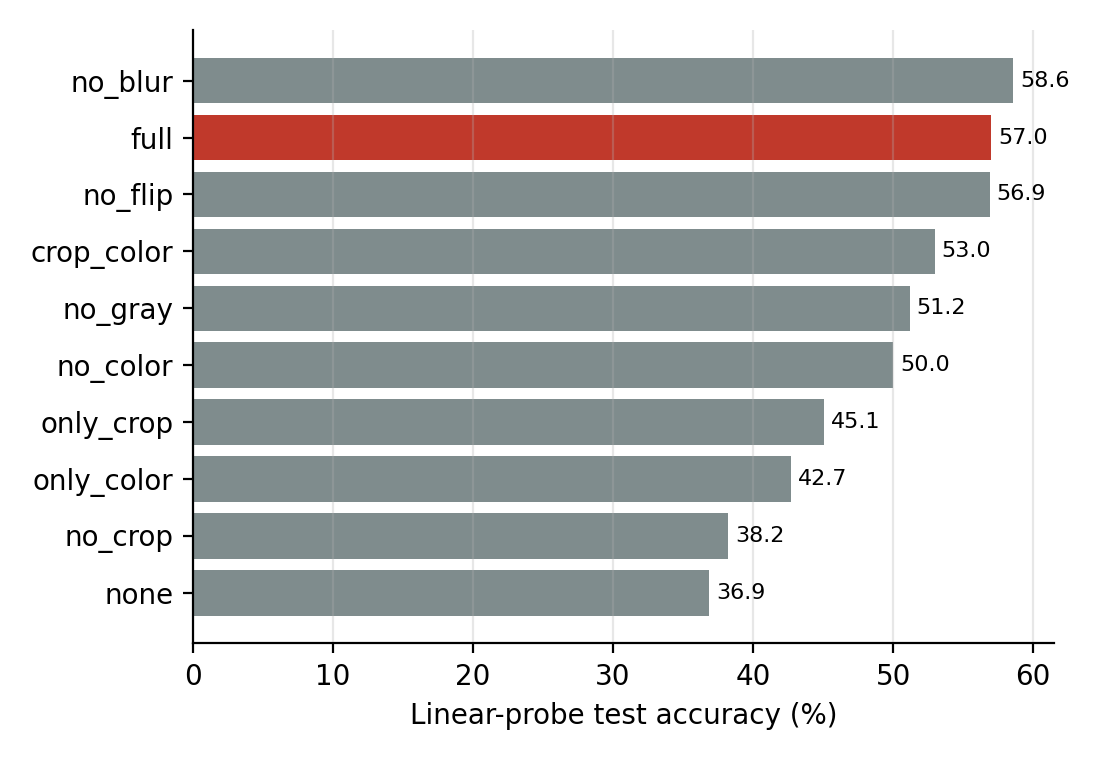
\includegraphics[width=0.65\linewidth]{aug_ablation.png}
  \caption{Linear-probe accuracy for each augmentation setting. The full set is highlighted.}
  \label{fig:aug}
\end{figure}

\paragraph{Crop matters most.} Ranked by the drop when one augmentation is removed: crop (18.8 points), colour
jitter (7.0), grayscale (5.8), flip (0.1) and blur ($-1.6$, so accuracy rose). Without crop, accuracy (38.2\%)
is almost the same as with no augmentation at all (36.9\%). Crop alone (45.1\%) is better than colour jitter
alone (42.7\%).

\paragraph{Colour jitter is second.} Adding colour jitter to crop raises accuracy from 45.1\% to 53.0\%
($+7.9$ points). This agrees with \citet{chen2020}, who found crop plus colour distortion to be the key pair:
without colour changes, two crops of one image can be matched by their colour statistics alone, so the network
learns less about shape and content. Grayscale, another colour distortion, also helps ($-5.8$ points when
removed).

\paragraph{Flip and blur did not help.} Removing flip changed accuracy by 0.1 points, and removing blur raised
it by 1.6 points. Possible reasons are that $96\times96$ images are already low in detail, so blur removes
useful information, and that a 20-epoch schedule may be too short to benefit from weaker augmentations. Both
differences are within what one seed can explain, so we read them as no benefit rather than harm.

\paragraph{Cost.} The augmentations run on the CPU, and data loading, not the GPU, limited training speed.
Within the same Kaggle session, 20 epochs took 944\,s with all augmentations, 645\,s without colour jitter and
357\,s with crop only. The no\_blur run took 633\,s but ran in a different session, so that comparison is only
indicative.

\paragraph{Answer for a small budget.} Use crop, flip, colour jitter and grayscale, and skip blur. That exact
set scored 58.6\%, slightly above the full set, and avoids the cost of blur.

% ---------------------------------------------------------------- 7. Batch-size ablation (Nidhi)
\section{Batch-size ablation}\label{sec:bs}
All augmentations are on, with the same 20 epochs and 20,000 images as above. The batch-256 point is the
\texttt{full} run of Section~\ref{sec:aug}.

\begin{table}[H]
  \centering
  \caption{Batch-size ablation. Linear-probe test accuracy (\%) and pretraining time for 20 epochs.}
  \label{tab:bs}
  \begin{tabular}{cccc}
    \toprule
    Batch size & Updates per epoch & Accuracy & Pretraining time (s) \\
    \midrule
    64  & 312 & \textbf{59.3} & 930 \\
    128 & 156 & 58.2 & 936 \\
    256 & 78  & 57.0 & 944 \\
    512 & 39  & 53.2 & 979 \\
    \bottomrule
  \end{tabular}
\end{table}

\begin{figure}[H]
  \centering
  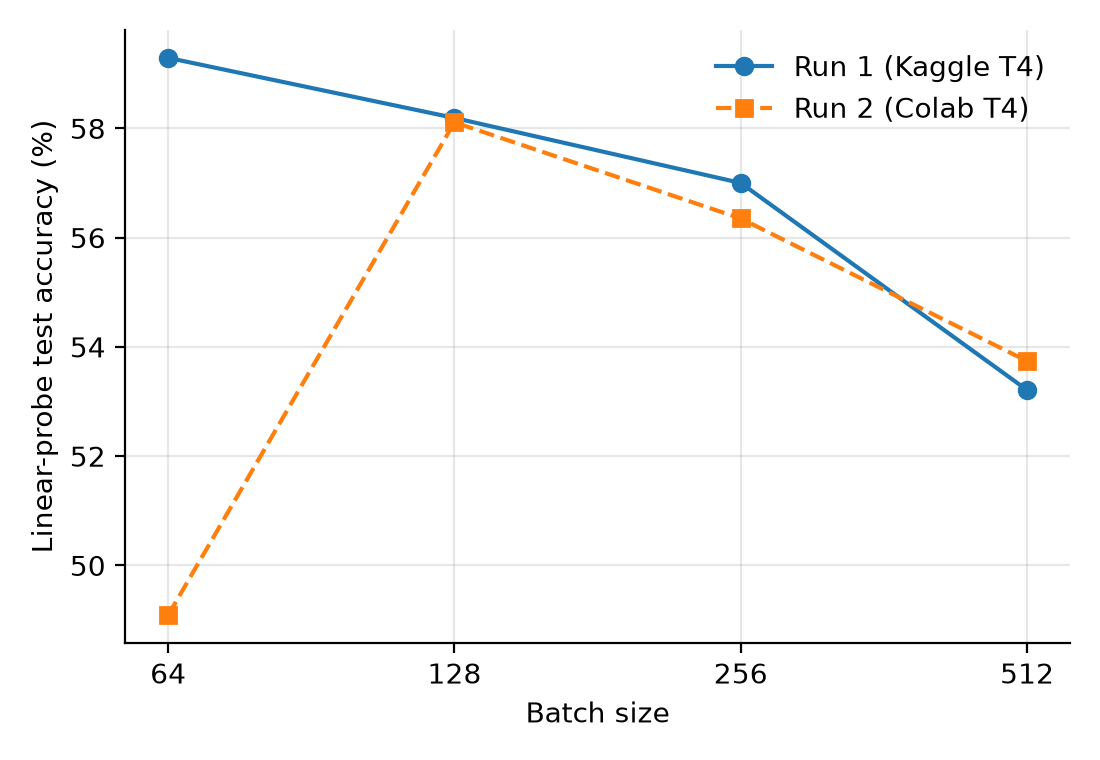
\includegraphics[width=0.6\linewidth]{batchsize_ablation.png}
  \caption{Linear-probe accuracy against pretraining batch size (20 epochs, 20,000 images).}
  \label{fig:bs}
\end{figure}

SimCLR reports that larger batches help because they give more negatives per step. On our budget the opposite
happened: accuracy fell from 59.3\% at batch size 64 to 53.2\% at 512 (Table~\ref{tab:bs},
Figure~\ref{fig:bs}). The likely reason is the number of updates. With a fixed 20 epochs, batch 512 makes only
39 updates per epoch against 312 for batch 64. The large-batch advantage in the paper appears with long
training (hundreds of epochs) and the LARS optimiser, neither of which we used. Run time was almost the same for
every batch size (930 to 979\,s), which again points to CPU data loading as the bottleneck. On a small budget, a
smaller batch is the better choice.

% ---------------------------------------------------------------- 8. Discussion (Shubham)
\section{Discussion and limitations}\label{sec:discussion}
SimCLR pretraining improved accuracy over the supervised baseline at every label fraction, and the
improvement grew as labels became scarcer. The ablations show that this benefit depends mostly on random
resized crop and colour distortions, and that on a short schedule small batches work better than large ones.

The main limitations are:
\begin{itemize}
  \item Short pretraining (50 epochs, against hundreds in the SimCLR paper), so absolute accuracies are lower
  than published results.
  \item The ablations use 20 epochs on a 20,000-image subset and one seed, so differences under about 2 points
  (flip and blur) may be noise.
  \item The ablations ran in two Kaggle sessions. Accuracy is unaffected, but run times are only fully
  comparable within one session.
  \item We used AdamW instead of LARS, and batch sizes up to 512 instead of up to 8,192.
  \item Only $96\times96$ images and a ResNet-18 were tested.
\end{itemize}

% ---------------------------------------------------------------- 9. Conclusion (Shubham)
\section{Conclusion}\label{sec:conclusion}
SimCLR pretraining on unlabelled STL-10 images improved accuracy over a supervised baseline at every label
fraction we tested (fine-tuning at 100\%, 20\% and 10\%, the linear probe at 1\%), with the largest gains when
labels were scarcest ($+21.2$ points at 10\% labels and $+26.2$ at 1\%). On a small compute budget, random
resized crop is the augmentation that matters most, followed by colour jitter and grayscale, while flip and blur
can be dropped without losing accuracy. Smaller batches worked better than larger ones at a fixed number of
epochs. Future work: longer pretraining, more seeds for the ablations, and the LARS optimiser with larger
batches.

% ---------------------------------------------------------------- Contributions
\section*{Contributions}
\begin{itemize}
  \item \textbf{Shubham Kang:} SimCLR implementation (data pipeline, augmentations, model, NT-Xent loss,
  training and evaluation scripts), the Kaggle setup and all pretraining and ablation runs, the augmentation
  ablation analysis, the method, discussion and conclusion sections, and assembly of the report.
  \item \textbf{Sandhya Parmar:} supervised baseline experiments, the fix for training at 1\% labels, the
  experimental setup and the baseline vs SimCLR results and analysis.
  \item \textbf{Nidhi:} introduction, related work, the batch-size ablation section, references and the
  repository documentation.
\end{itemize}

% ---------------------------------------------------------------- References
\begin{thebibliography}{99}
\bibitem[Chen et~al.(2020)]{chen2020}
T.~Chen, S.~Kornblith, M.~Norouzi and G.~Hinton.
\newblock A simple framework for contrastive learning of visual representations.
\newblock In \emph{ICML}, 2020. \url{https://arxiv.org/abs/2002.05709}

\bibitem[Coates et~al.(2011)]{coates2011}
A.~Coates, A.~Ng and H.~Lee.
\newblock An analysis of single-layer networks in unsupervised feature learning.
\newblock In \emph{AISTATS}, 2011.

\bibitem[Gidaris et~al.(2018)]{gidaris2018}
S.~Gidaris, P.~Singh and N.~Komodakis.
\newblock Unsupervised representation learning by predicting image rotations.
\newblock In \emph{ICLR}, 2018.

\bibitem[He et~al.(2016)]{he2016}
K.~He, X.~Zhang, S.~Ren and J.~Sun.
\newblock Deep residual learning for image recognition.
\newblock In \emph{CVPR}, 2016.

\bibitem[He et~al.(2020)]{he2020}
K.~He, H.~Fan, Y.~Wu, S.~Xie and R.~Girshick.
\newblock Momentum contrast for unsupervised visual representation learning.
\newblock In \emph{CVPR}, 2020.

\bibitem[Krizhevsky et~al.(2012)]{krizhevsky2012}
A.~Krizhevsky, I.~Sutskever and G.~Hinton.
\newblock ImageNet classification with deep convolutional neural networks.
\newblock In \emph{NeurIPS}, 2012.

\bibitem[Loshchilov and Hutter(2019)]{loshchilov2019}
I.~Loshchilov and F.~Hutter.
\newblock Decoupled weight decay regularization.
\newblock In \emph{ICLR}, 2019.

\bibitem[Noroozi and Favaro(2016)]{noroozi2016}
M.~Noroozi and P.~Favaro.
\newblock Unsupervised learning of visual representations by solving jigsaw puzzles.
\newblock In \emph{ECCV}, 2016.

\bibitem[van~den Oord et~al.(2018)]{oord2018}
A.~van~den Oord, Y.~Li and O.~Vinyals.
\newblock Representation learning with contrastive predictive coding.
\newblock \emph{arXiv:1807.03748}, 2018.

\bibitem[Silva(2020)]{silva2020}
T.~S.~Silva.
\newblock PyTorch SimCLR: a simple framework for contrastive learning of visual representations.
\newblock GitHub repository, 2020. \url{https://github.com/sthalles/SimCLR}

\bibitem[Wu et~al.(2018)]{wu2018}
Z.~Wu, Y.~Xiong, S.~Yu and D.~Lin.
\newblock Unsupervised feature learning via non-parametric instance discrimination.
\newblock In \emph{CVPR}, 2018.

\bibitem[You et~al.(2017)]{you2017}
Y.~You, I.~Gitman and B.~Ginsburg.
\newblock Large batch training of convolutional networks.
\newblock \emph{arXiv:1708.03888}, 2017.

\bibitem[Zhang et~al.(2016)]{zhang2016}
R.~Zhang, P.~Isola and A.~A.~Efros.
\newblock Colorful image colorization.
\newblock In \emph{ECCV}, 2016.
\end{thebibliography}

\end{document}
